\chapter{Beech Forests}

The second major forest type\footnote{\cite{wardle1984beeches}} in New Zealand provides a strong contrast to the conifer broadleaf forest.
It is dominated in the canopy or forest `roof' by one or more species of southern beech (\BotanicRef{Nothofagus}),\footnote{\BotanicRef{Nothofagus} means `false beech'.} a genus restricted to the southern hemisphere, but nevertheless related to the oaks and true beeches (\BotanicRef{Fagus}) of the northern hemisphere. \BotanicRef{Fagus} and \BotanicRef{Nothofagus} are largely distinguished by flower and fruit characteristics, but in addition the New Zealand species of \BotanicRef{Nothofagus}, and a number elsewhere, differ from \BotanicRef{Fagus} in being evergreen and having much smaller leaves.
However, despite the clear differences between the two genera, it has become customary in New Zealand to refer to our species as `beech' without qualification.

\section{Species and Varieties of New Zealand Beech}

Five species of \BotanicRef{Nothofagus} were formerly recognised in New Zealand, but more recently two of these have been combined as varieties of one species.\footnote{\cite{poole1958studies}}

\begin{itemize}
	\item \BotanicRef{Nothofagus menziesii}[Nothofagus][menziesii]: \IDX{silver beech}[beech!silver] (the bark is white and silvery particularly in young trees).
	\item \BotanicRef{Nothofagus fusca}[Nothofagus][fusca]: \IDX{red beech}[beech!red] (the timber is reddish in colour).
	\item \BotanicRef{Nothofagus truncata}[Nothofagus][truncata]: \IDX{hard beech}[beech!hard] (the wood has a high silica content making it hard).
	\item \BotanicRef{Nothofagus solandri var.\ solandri}[Nothofagus][solandri var.\ solandri]: \IDX{black beech}[beech!black] (the bark is very dark partly due to the growth of a sooty mould).
	\item \BotanicRef{Nothofagus solandri var.\ cliffortioides}[Nothofagus][solandri var.\ cliffortioides]: \IDX{mountain beech}[beech!mountain] (grows mainly at higher altitudes than the other beeches).
\end{itemize}

\begin{SCfigure}[1.5][!b]
	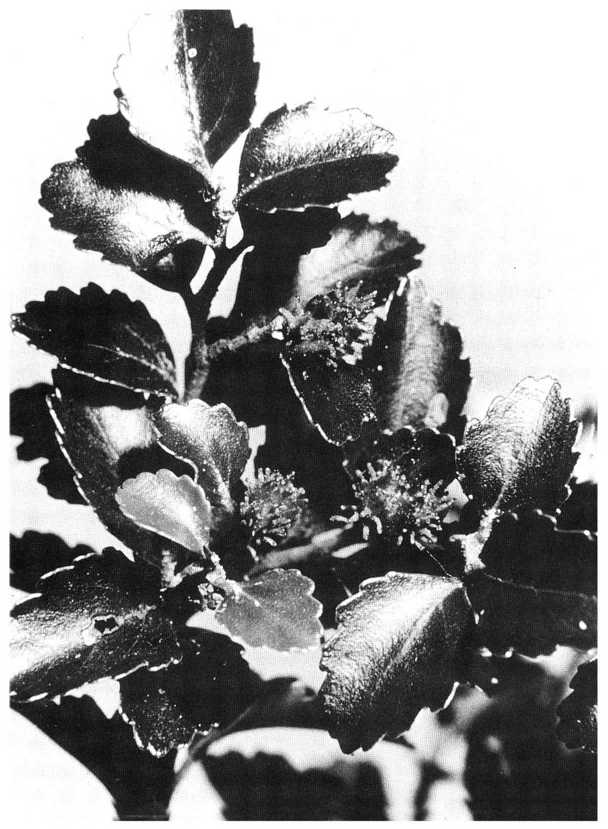
\includegraphics[width=0.4\textwidth]{graphics/figure69silverbeech.jpg}
	\centering
	\caption[Silver beech foliage and young fruits]{Silver beech foliage and young fruits with glandular hairs.
	Photo: M. D. King.}%
	\label{fig:69silverbeech}
\end{SCfigure}

\IDX{Silver beech}[beech!silver] has thick, almost circular leaves, \SIrange{0.5}{1.5}{\centi\metre} long and wide, bearing a few domatia on the underside and small, rounded marginal teeth often in pairs\figureref{\fullref{fig:69silverbeech}}.
The leaves of red and \IDX{hard beech}[beech!hard] are similar to each other, \SIrange{2}{4}{\centi\metre} long by \SIrange{1.5}{2.5}{\centi\metre} wide and with saw-like marginal teeth.
\IDX{Hard beech}[beech!hard] has rather thicker leaves with 8 to 12 teeth per side compared with 6 to 8 for red beech; \IDX{red beech}[beech!red] alone has domatia.
Black and \IDX{mountain beech}[beech!mountain] have small smooth-margined leaves, hairy below, \SIrange{1}{1.5}{\centi\metre} long by \SIrange{0.5}{1}{\centi\metre} wide.
It is difficult to distinguish the leaves of the last two forms.
\IDX{Mountain beech}[beech!mountain] at higher altitudes often has leaves that taper from the base, while the leaves of \IDX{black beech}[beech!black] at low altitudes are oblong, but there are intergrading forms in many places.

Silver, hard and \IDX{red beech}[beech!red] may become large trees \SI{30}{\metre} or more in height with trunks \SI{2}{\metre} or more in diameter.
The trunk bases of the first two have low, rounded buttresses while those of the latter are high and narrow.
The larger trees of mountain and \IDX{black beech}[beech!black] are generally below \SI{25}{\metre} in height with unbuttressed trunks of about \SI{1}{\metre} in diameter.

The bark of all the beeches, except when young, is rough and fissured.
The tree crowns, especially in more open situations, are wide and deep and particularly in mountain and \IDX{black beech}[beech!black], the foliage is often arranged in distinctive horizontal layers.
The male and female flowers at the tips of twigs are wind-pollinated and inconspicuous, although in good flowering years coloured anthers in the male flowers may impart a reddish glow to the crowns of black and \IDX{mountain beech}[beech!mountain] particularly.
More brilliant splashes of colour, contrasting with the dark green of the foliage, may be provided by certain mistletoes which commonly parasitise the beeches.
\IDX{Scarlet mistletoe}[scarlet mistletoe] (\BotanicRef{Peraxilla colensoi}[Peraxilla][colensoi], \IDX{korukoru}, \IDX{pirita}, \IDX{roeroe}), usually found on \IDX{silver beech}[beech!silver], and \IDX{red mistletoe} (\BotanicRef{Peraxilla tetrapetala}[Peraxilla][tetrapetala], \IDX{pikirangi}, \IDX{pirita}, \IDX{roeroe}, \IDX{pirinoa}) have bright red flowers.
\IDX{Yellow mistletoe} (\BotanicRef{Alepis flavida}[Alepis][flavida], \IDX{pirita}, \IDX{piriraki}) with orange-yellow to yellow flowers used to be common, but has now been depleted by opossums.
Heavy flowering of all the beech species in New Zealand takes place every few years with little or no flowering in the other years.
It is suggested that `flowering years' follow hot summers which encourage the initiation of flower buds.\footnote{\cite{poole1948flowering}}

The beech seed are \SIrange{5}{8}{\milli\metre} long with narrow wings.
It is considered that they are not capable of being dispersed for more than a few kilometres and then only with strong winds.\footnote{\cite{preest1963dispersal}}

\IDX{Silver beech}[beech!silver] stands apart from the other species in several respects.
Some of the more striking differences are:

\begin{description}
	\item[{(a)}]each leaf of a \IDX{silver beech}[beech!silver] generally lasts several years before falling, those of the other species last for only one year, generally falling a few weeks after the new season's leaves have unfolded, or even, in the cases of occasional trees of red and \IDX{hard beech}[beech!hard], a few weeks before;
	\item[{(b)}]natural hybrids have often been observed involving all species except silver beech;
	\item[{(c)}]silver beech is the only species attacked by a fungus, \BotanicRef{Cyttaiia}, whose orangey, golf-ball-like fruiting bodies may be abundant on the branches of some trees;
	\item[{(d)}]study of the pollen of the New Zealand beeches has shown that \IDX{silver beech}[beech!silver] has a different form of grain from that shared by the other species.
\end{description}

\begin{SCfigure}[1.0][t]
	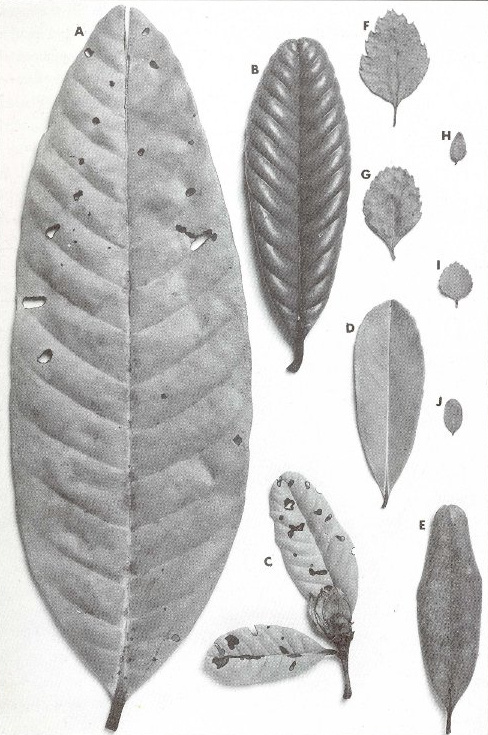
\includegraphics[width=0.5\textwidth]{graphics/figure70nothofagus.jpg}
	\centering
	\caption[New Zealand and New Caledonian Nothofagus leaves]{New Zealand and New Caledonian \BotanicRef{Nothofagus} leaves.
	\IDX{New Caledonia}: \BotanicRef{Nothofagus codanandra}[Nothofagus][codanandra];
	A, juvenile leaf;
	B, adult leaf;
	C, twig with a cupule with 3 flat seeds;
	D, \BotanicRef{Nothofagus sp.}[Nothofagus];
	E, \BotanicRef{Nothofagus equilateralis}[Nothofagus][equilateralis].
	New Zealand:
	F, \IDX{red beech}[beech!red] (\BotanicRef{Nothofagus fusca}[Nothofagus][fusca]);
	G, \IDX{hard beech}[beech!hard] (\BotanicRef{Nothofagus truncata}[Nothofagus][truncata]);
	H, \IDX{mountain beech}[beech!mountain] (\BotanicRef{Nothofagus solandri var.\ cliffortioides}[Nothofagus][solandri var.\ cliffortioides]);
	I, \IDX{silver beech}[beech!silver] (\BotanicRef{Nothofagus menziesii}[Nothofagus][menziesii]);
	J, \IDX{black beech}[beech!black] (\BotanicRef{Nothofagus s.\ var.\ solandri}[Nothofagus][s.\ var.\ solandri]).
	Photo: M. D. King.}%
	\label{fig:70nothofagus}
\end{SCfigure}

For the last reason our species have been assigned to two informal groups within the genus, both of which are also represented in Australia and South America --- the `menziesii group' and the `fusca group'.
A third `brassii group', with a third pollen type, is restricted at present to New Caledonia\figureref{\fullref{fig:70nothofagus}} and New Guinea.\footnote{\cite{cranwell1939southern}}

\section{Structure and Composition of New Zealand Beech Forests}

\begin{figure}[t]
	% Outer minipage scaled to limit width.
	% Inner minipages scaled so the images have the same height.
	\begin{minipage}[t]{\textwidth}
		\begin{minipage}[t]{(\textwidth-\fgap) * \real{0.501}}
			\centering
			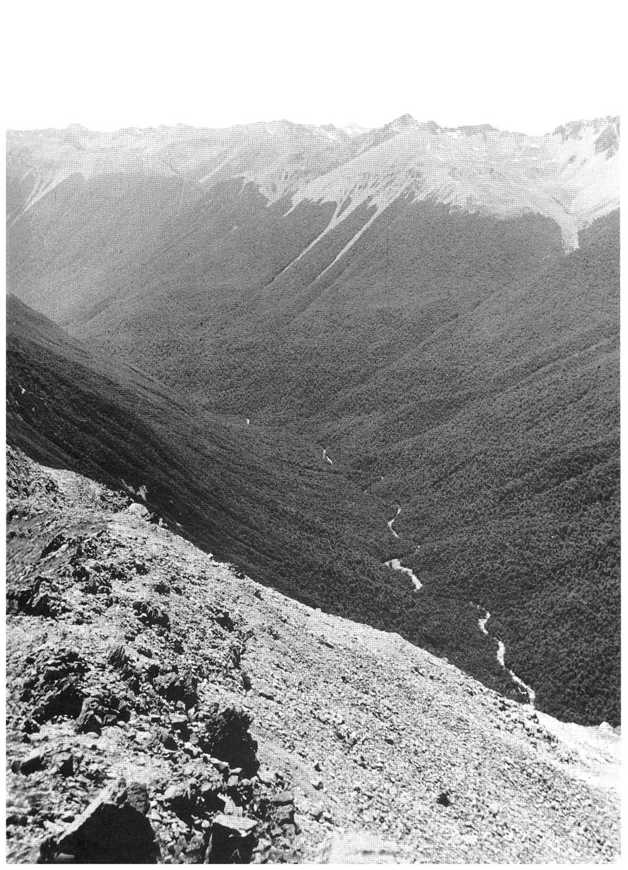
\includegraphics[width=\textwidth]{graphics/figure71nothofagus-forest.jpg}
			\caption[Nothofagus forest in the Travers Valley]{\BotanicRef{Nothofagus} forest in the Travers Valley, northern South Island.
			Note the even treeline.
			Photo: J. W. Dawson.}%
			\label{fig:71nothofagus-forest}
		\end{minipage}\hspace{\fgap}%
		\begin{minipage}[t]{(\textwidth-\fgap) * \real{0.499}}
			\centering
			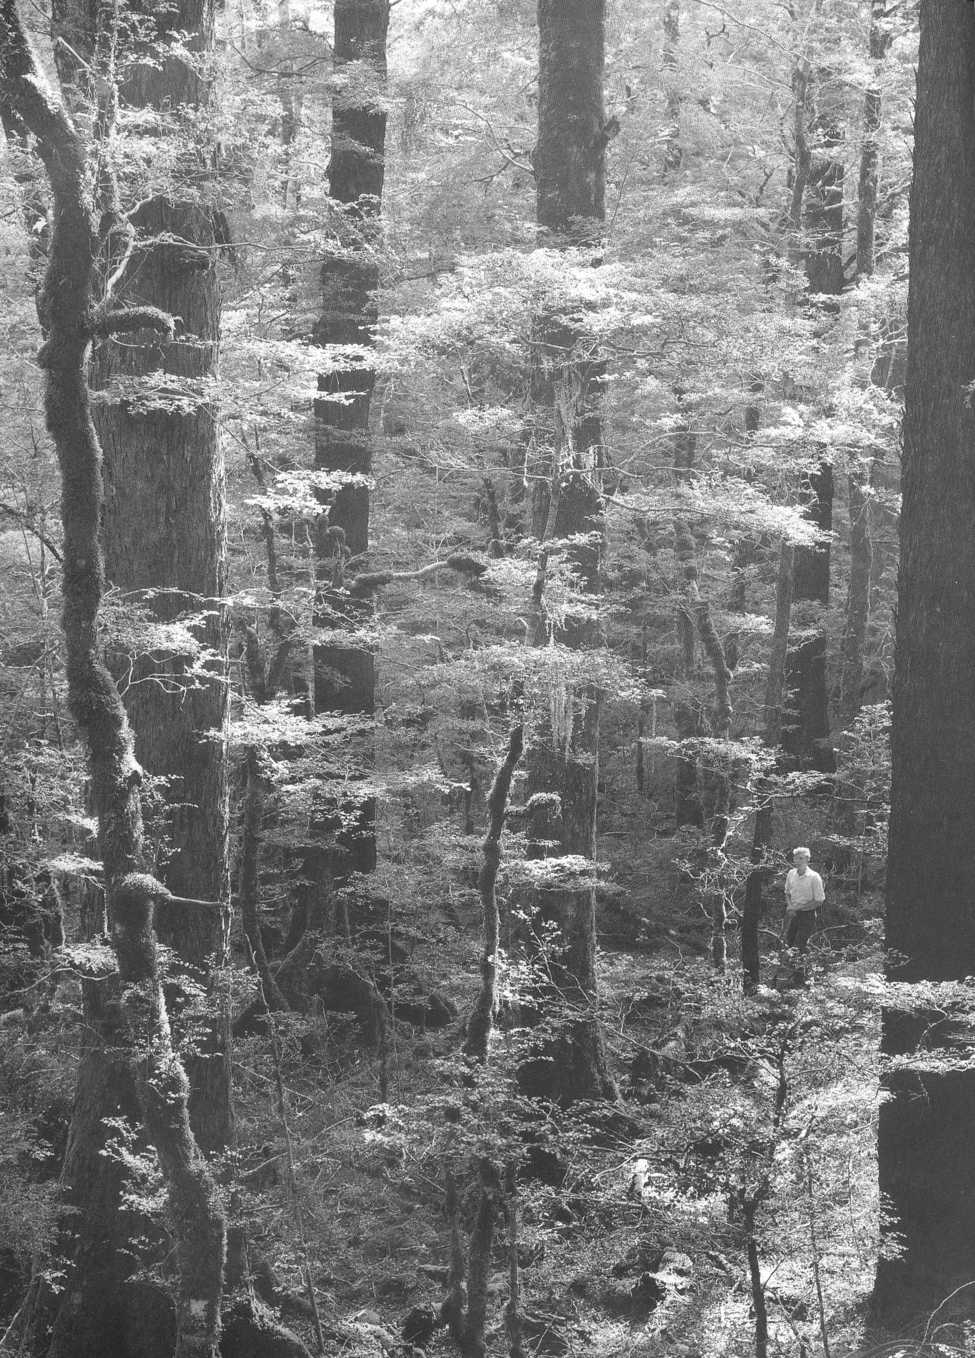
\includegraphics[width=\textwidth]{graphics/figure72beech.jpg}
			\caption[Interior of red beech and silver beech forest]{Interior of \IDX{red beech}[beech!red] (\BotanicRef{Nothofagus fusca}[Nothofagus][fusca]) and \IDX{silver beech}[beech!silver] (\BotanicRef{Nothofagus menziesii}[Nothofagus][menziesii]) forest near the Maruia Saddle, South Island.
			Photo: J. H. Johns.}%
			\label{fig:72beech}
		\end{minipage}
	\end{minipage}
\end{figure}

Seen from either the inside or the outside, pure beech forest in New Zealand has a very different appearance from conifer broadleaf forest.
Externally\figureref{\fullref{fig:71nothofagus-forest}}, for example when viewed on the steep side of a mountain valley, beech forest has a uniform, generally dark green colour and a smooth to moderately uneven surface.
There are no emergent j trees.
There is none of the tangled profusion of the conifer broadleaf forest within the beech forest\figureref{\fullref{fig:72beech}}, particularly when rainfall is moderate or low.
There are clearly fewer species present and because of the sparse undergrowth and absence of vines, one can walk freely among the rough-barked trunks.
Vascular epiphytes too are generally absent, although there are often epiphytic mosses and lichens on the trunks and branches.
The forest floor has a deep carpet of leaf litter, soft cushions of the pale green \IDX{milk moss} (\BotanicRef{Leucobryum candidum}[Leucobryum][candidum]) and masses of the translucent fans of the \IDX{kidney fern} (\BotanicRef{Trichomanes reniforme}[Trichomanes][reniforme]).
Among the scattered shrubs which may be present, the small leaved \IDX{mingimingi} (\BotanicRef{Styphelia fasciculata}[Styphelia][fasciculata]) (Cyathodes), \IDX{prickly mingimingi} (\BotanicRef{Styphelia juniperina}[Styphelia][juniperina]), \BotanicRef{Coprosma rhamnoides}[Coprosma][rhamnoides] and \BotanicRef{Coprosma microcarpa}[Coprosma][microcarpa] are most frequently encountered.
Light filtering through the attractive layers of the beech foliage contributes to the typically tranquil, orderly atmosphere of this type of forest.
Beech forest becomes more complex with higher rainfall, as on the west of mountains at higher altitudes.
Its growth appears more luxuriant, largely as a result of the profusion of lichens, mosses, liverworts and moss-like filmy ferns clothing the forest floor and trunks and branches of the trees.
Where the canopy is partly open there are also more species of small trees and shrubs involved although none is restricted to beech forests.
\IDX{Broadleaf}[broadleaf] (\BotanicRef{Griselinia littoralis}[Griselinia][littoralis], \IDX{kapuka}, \IDX{papauma}), \IDX{haumakoroa} (BotanicRef{Pseudopanax simplex}[Pseudopanax][simplex]), \IDX{stinkwood} (\BotanicRef{Coprosma foetidissima}[Coprosma][foetidissima]) and others may contribute to a subcanopy and there is often a shrub layer of small-leaved coprosmas, the smallleaved \IDX{weeking matipo} (\BotanicRef{Myrsine divaricata}[Myrsine][divaricata]), the mountain \IDX{horopito} (\BotanicRef{Pseudowintera colorata}[Pseudowintera][colorata]) and others.

Larger ferns on the forest floor include the well-known \IDX{crepe fern} or Prince of Wales Feathers (\BotanicRef{Leptopteris superba}[Leptopteris][superba], \IDX{heruheru}) and \IDX{crown fern} (\BotanicRef{Blechnum discolor}[Blechnum][discolor], \IDX{petipeti}, \IDX{piupiu}).
Two small flowering plants growing in moss cushions are characteristic of this type of forest --- \BotanicRef{Luzuriaga parviflora}[Luzuriaga][parviflora] with spreading wiry stems, two-ranked leaves and large spongy white berries, and \IDX{mikoikoi} (\BotanicRef{Libertia pulchella}[Libertia][pulchella]) with half erect fans of grasslike leaves.

These wet beech forests in New Zealand are sometimes swathed in mist; forests of a similar character elsewhere in the world are often referred to as cloud or mossy forest, or more romantically `goblin forest' or `elfin woodland'.

At the other extreme, some of the beech forests in relatively dry sites on the east of the South Island mountain axis are among the simplest of forests anywhere, consisting of virtually a single species --- \IDX{mountain beech}[beech!mountain].

As a generalisation, where there is a trend away from mild, moist conditions and fertile soils towards cooler or drier conditions and less fertile soils, or combinations of these, there is often a transition from conifer broadleaf to beech forest.

\section{Lowland Beech Forest}

\IDX{Black beech}[beech!black] and \IDX{hard beech}[beech!hard] are often referred to as the lowland beeches because they are generally found in the same altitudinal zone as the conifer broadleaf forest.
They reach their southern limits in the northern South Island, with a disjunct occurrence of \IDX{hard beech}[beech!hard] in south Westland.

\begin{SCfigure}[0.5][!b]
	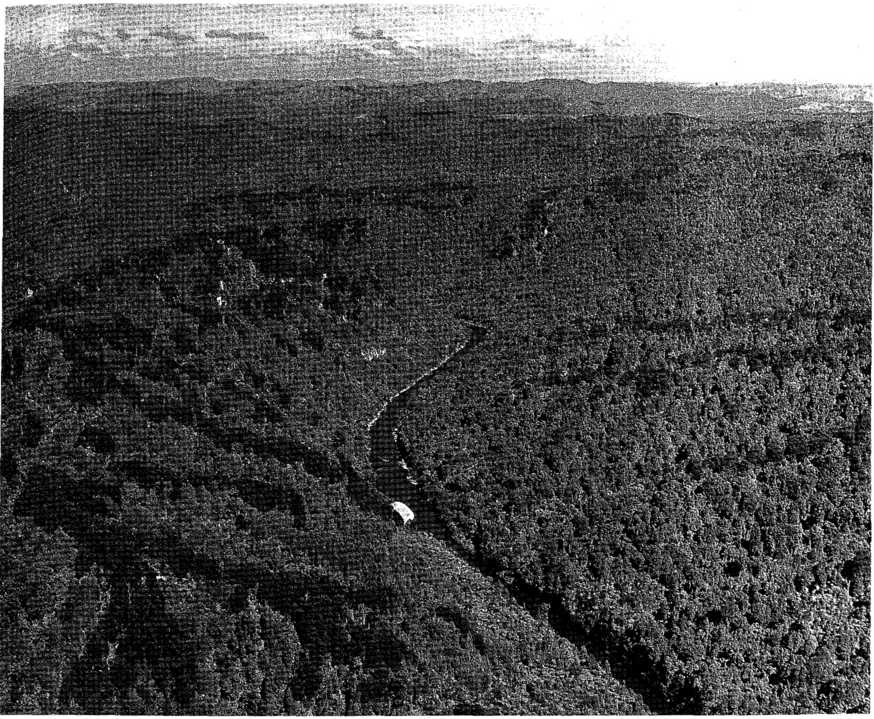
\includegraphics[width=0.66\textwidth]{graphics/figure73taranaki-forests.jpg}
	\centering
	\caption[Aerial view of inland Taranaki forests]{Aerial view of inland Taranaki forests with strips of dark-coloured lowland beech forest on the ridges and conifer broadleaf forest on the slopes and in the valleys.
	Photo: White's Aviation.}%
	\label{fig:73taranaki-forests}
\end{SCfigure}

The lowland beeches generally do not become components of the conifer broadleaf forest, however, but form instead mainly narrow strips of forest on the thin, stony, infertile soils of ridge crests\figureref{\fullref{fig:73taranaki-forests}} or cliff edges.
Often the change from dense conifer broadleaf forest to open beech forest is very abrupt.
In the steepest, stoniest and driest sites only \IDX{black beech}[beech!black] may be present\footnote{Black beech and its relative \IDX{mountain beech}[beech!mountain] are both tolerant of dry conditions, but can also grow on poorly drained swampy sites. This is not as anomalous as it seems, as poorly drained soils are considered to be `physiologically dry' as the lack of free oxygen greatly reduces the water absorption efficiency of the roots.} but elsewhere the two species may intermingle or, on somewhat better soils, \IDX{hard beech}[beech!hard] may predominate.

\section{Montane Beech Forest}

In many places in New Zealand, conifer broadleaf forest gives way at higher elevations to a beech forest dominated by one or more of the montane beeches --- red, silver or mountain.
This occurs because of the decrease of temperature as altitude increases.
Naturally the altitudes at which the transition takes place varies with latitude: at \SIrange{38}{39}{\degree}S from East Cape to the central North Island it ranges from about \SIrange{850}{1000}{\metre}; at \ang{41}S in the southern North Island it is at about 750 m; at \ang{45}S in the south-west South Island it is at about 450 m; and at the southern end of the South Island at \ang{46}S, montane beech forest approaches sea level in places.

The three montane beech species differ ecologically.
\IDX{Red beech}[beech!red] gives way to \IDX{silver beech}[beech!silver], which gives way to \IDX{mountain beech}[beech!mountain] as temperatures become colder and soils become thinner and less fertile.
Thus if the three occur together on the same mountain, \IDX{red beech}[beech!red] often dominates immediately above the conifer broadleaf forest giving way upwards to \IDX{silver beech}[beech!silver], which in turn gives way to \IDX{mountain beech}[beech!mountain] towards the treeline.

\IDX{Mountain beech}[beech!mountain] is also more tolerant of drier conditions than the other two species so on the drier eastern sides of the mountain ranges, particularly in the South Island, it is often the only beech species present pr even virtually the \emph{only} tree species present as already mentioned.
Conversely, on wetter sites, for example to the west of the mountain ranges, \IDX{mountain beech}[beech!mountain] becomes much less common or absent and its place at treeline may be taken by \IDX{silver beech}[beech!silver].

\section{Treeline}

Where beech forest is present and when temperatures become too cold for tree growth as the altitude increases, there is often an abrupt change from the uppermost trees to a vegetation of alpine herbs and/or shrubs.

The highest treelines are those where \IDX{mountain beech}[beech!mountain] is present.
In the central North Island at \ang{39}S the \IDX{mountain beech}[beech!mountain] treelines range from about \SIrange{1350}{1500}{\metre}; in the north-eastern South Island at \ang{42}S, \SIrange{1300}{1550}{\metre}; and in the southern South Island at \ang{45}S from \SIrange{950}{1250}{\metre}.

Compared with treelines at comparable latitudes on a continent, those in New Zealand are unusually low.\footnote{\cite{wardle1965comparison}}\footnote{\cite{wardle1971explanation}} For example, at \ang{39}N in the Rocky Mountains of North America, the treeline can be as high as \SI{3630}{\metre}, This apparent anomaly seems to relate to the difference in summer temperatures between continents and islands at comparable latitudes.
Land heats up much more in summer than the sea, so a continent will attain higher temperatures at given latitudes and altitudes than a narrow island surrounded by the relatively cooler sea.
Consequently vegetation zone boundaries, including the treeline, are higher on continents than on islands.
It is estimated that a mean warmest month temperature of \ang{10}C determines the upper limit of tree growth and this seems to hold as true for the relatively low beech treelines in New Zealand as for the higher continental treelines.

On this basis it might be expected that mountains furthest from the sea in New Zealand with more `continental' climates would have higher treelines.
This proves to be the case.
The highest treelines in New Zealand are on Mt Ruapehu in the central North Island (ca. \SI{1500}{\metre}) and on the mountains at the centre of the northern South Island (ca. \SI{1550}{\metre}).
Inverted treelines occur where there are flat valley floors not far below the normal treeline.
In frosty weather the coldest air sinks to the valley floor, which as a result experiences much lower temperatures than the valley sides, despite their higher altitude.
In these circumstances the valley floor is occupied by an open vegetation of an alpine/subalpine character, while the slopes support forest.

\section{Beech Gaps}

There are regions in New Zealand where beech species are completely absent, even though at appropriate altitudes conditions seem entirely suitable for them.
Such regions are: Mt Taranaki (Egmont), an isolated volcanic cone in the west of the North Island; the southern Ruahines and adjacent northern Tararuas in the south of the North Island; in the South Island, a strip to the west of the high central third of the mountain axis (Westland) with a narrower gap on the east; and Fiordland.
For the central South Island at least it is suggested that beech was eliminated there during the last glaciation and because of its slow rate of dispersal has not yet fully reinvaded from southern and northern refugia.\footnote{\cite{wardle1965comparison}}
As a consequence more readily dispersing conifer broadleaf forest species have established in sites perhaps better suited to beech species particularly at higher elevations. (See Chapter 12 for further discussion of the discontinuous distributions (disjunctions) of the beeches and other native species.)

\section{Intermediate Forest Types}

Forests comprising mixtures of conifer broadleaf forest species (particularly the conifers) and beech can be found throughout New Zealand.
In the north of the North Island there are even a few localities where \IDX{hard beech}[beech!hard] intermingles with \IDX{kauri} (\BotanicRef{Agathis}).

Such intermediate forests may be found in the transition from conifer broadleaf forest to pure beech forest on mountain slope, but to the north and south of the Westland beech gap, there are more extensive mixed forests at lower and middle elevations.
Some workers have suggested that this results from the slow replacement by advancing beech forest of the Westland conifer broadleaf forest.\footnote{\cite{holloway1954forests}}\footnote{\cite{wardle1964facets}}\footnote{\cite{wardle1980ecology}}

\section{Beech Forest Regeneration}

The species of southern beech are all relatively light-demanding.
Seedlings may establish on better-lit parts of the forest floor but then `stand still' until more light is available from the death of a canopy tree or as a result of more extensive openings caused by violent gales.
Such openings or clearings may soon be filled by a dense `crop' of vigorous young beech trees.

Where beech forest is destroyed by fire followed by the establishment of \IDX{manuka} and/or \IDX{kanuka}, then there is sufficient light at ground level for beech to become established, grow strongly and, in time, to overtop and shade out the pioneers.

\subsection{Relationships of the New Zealand Beech Forests}

Unlike the New Zealand conifer broadleaf forest, beech forest shows few similarities with tropical rain forest.
Indeed its simpler structure fewer species and general lack of vascular epiphytes and lianes, linked with the relationship of the dominant trees with true beech of the northern hemisphere, might indicate a vegetational affinity with north temperate deciduous forest.

New Zealand beech forest, however, differs from north temperate deciduous forest in certain respects.
The leaves of the trees are evergreen and relatively small.
The forest generally occupies infertile sites and forms a slowly decomposing, low-nutrient leaf litter which, because of its acidity, accelerates leaching and further reduces soil fertility.
North temperate deciduous forest, on the other hand, generally occupies more fertile soils and forms a rapidly decomposing leaf litter, high in nutrients, which tends to improve the fertility of the soil.

In the respects in which New Zealand and other southern hemisphere beech forests differ from north temperate deciduous forest, there is a fair measure of agreement with the vast coniferous forests of high northern latitudes.
This has led to the suggestion that these two forest types of cooler infertile sites in the two hemispheres are approximate ecological equivalents.\footnote{\cite{dansereau1964six}}

However, as there are a number of deciduous species of \BotanicRef{Nothofagus} in South America and one in Tasmania, it might be truer to say that \BotanicRef{Nothofagus} forest lies somewhere between the north temperate deciduous and coniferous forests.
Within New Zealand, in terms of nutrient demand and leaf size, \IDX{red beech}[beech!red] would come closest to the former and \IDX{mountain beech}[beech!mountain] to the latter.
